\documentclass[reqno]{amsart}
\usepackage[numbers]{natbib}
\usepackage{amssymb,mathtools,hyperref,graphicx,caption,gensymb}
\usepackage{subcaption}
\usepackage[export]{adjustbox}
\usepackage{wrapfig}
\graphicspath{ {images/} }
\hypersetup{colorlinks,linkcolor={blue},citecolor={red},urlcolor={blue}}
\newtheorem{theorem}{Theorem}[section]
\newtheorem*{theoremLESS}{Theorem 1.1}
\newtheorem{case}{Case}
\newtheorem{lemma}[theorem]{Lemma}
\newtheorem{proposition}[theorem]{Proposition}
\newtheorem{corollary}[theorem]{Corollary}
\theoremstyle{definition}
\newtheorem{definition}[theorem]{Definition}
\newtheorem{notation}[theorem]{Notation}
\numberwithin{equation}{section}
\newcommand{\bR}{\mathbb{R}}
\newcommand{\bQ}{\mathbb{Q}}
\newcommand{\bZ}{\mathbb{Z}}
\newcommand{\bN}{\mathbb{N}}
\newcommand{\bC}{\mathbb{C}}

\begin{document}
\title[Constructible Regular Polygons]{Infinite Sets of Constructible Regular Polygons}
\author{Katherine}
\date{May 11, 2022.}
\begin{abstract}This paper will investigate constructibility within regular $n$-gons and identify infinite sets of constructible and nonconstructible regular polygons. This topic stems from Ancient Greek mathematicians who sought to understand these geometric properties using the tools that they had.\end{abstract}
\maketitle
\section{Introduction to Constructibility}\label{sec:1}
Straightedge and compass constructions are points, lines, and shapes that can be drawn precisely by hand following a certain set of rules. The only two tools that can be used are straightedge to draw lines, and a compass that can draw circular arcs, however neither is able to preserve or measure distance. It is the Ancient Greek mathematicians who gave us these rules, for they were deeply curious about geometric constructions. There are three basic constructions that can be done:
\begin{enumerate}
  \item A straight line between two points.
  \item An extension of a given straight line.
  \item A circle centered at a given point with a given radius.
\end{enumerate}

From these three basic constructions, we can create all other constructions. We say that any point is constructible if and only if there exists a finite number of steps using these three basic constructions to reach that point. Likewise, the same is true for lines and polygons. Recall that a polygon with $n$ sides is simply referred to as an $n$-gon. We say that a polygon is regular if it it is equiangular (all angles are equal) and equilateral (all side lengths are equal), and we say that a polygon is irregular otherwise.

Constructing an irregular $n$-gon for any $n$ is trivial, however the same cannot be said for regular $n$-gons, as their complexity only grows. The Ancient Greek mathematicians knew how to construct regular $n$-gons for $n = 3,4,5$, along with how to construct a polygon with double the number of sides of a given polygon \cite{Bold}. Beyond this, the constructability of regular polygons was a mystery for thousands of years. The capstone of this paper will be in Section \ref{sec:4} where we prove the following:
\begin{theorem}\label{thm:gauss}A regular n-gon is constructible if and only if n is of the form $$n = 2^kp_1p_2....p_i$$ where $k \ge 0$ and $p_1,p_2,...p_i$ are distinct Fermat primes (primes of the form $2^{2^q} + 1$ for $q \in \bZ^+)$.\end{theorem}

\section{Constructing a Regular Triangle}\label{sec:2}

As a simple example to show how constructions work, we will show the construction of a regular triangle.
\begin{enumerate}
    \item First, draw a line segment $\overline{AB}$.
    \item Then, center a circle at point $A$ with radius $|AB|$, and draw an arc above the line segment $\overline{AB}$. Repeat this process with a circle centered at $B$ as well.
    \item Call the intersection of the two arcs point $C$. Draw $\overline{AC}$ and $\overline{BC}$ to finish.
\end{enumerate}
\begin{figure}[h]
\centering
\begin{subfigure}{0.3\textwidth}
\centering
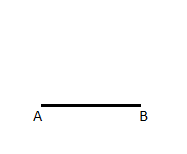
\includegraphics[scale=0.7]{step1.png}
\caption{Step 1}
\label{fig:subim1}
\end{subfigure}
\begin{subfigure}{0.3\textwidth}
\centering
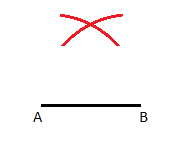
\includegraphics[scale=0.7]{step2.png}
\caption{Step 2}
\label{fig:subim2}
\end{subfigure}
\begin{subfigure}{0.3\textwidth}
\centering
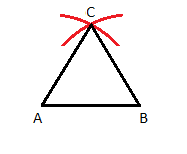
\includegraphics[scale=0.7]{step3.png}
\caption{Step 3}
\label{fig:subim3}
\end{subfigure}
\caption{Construction of the triangle}
\label{fig:1}
\end{figure}

The proof that $\triangle ABC$ is regular, ie that each interior angle is $60\degree$ and each side length is equal, is rather trivial. Because the radius for each arc is $|AB|$, the length of $\overline{AC}$ and $\overline{BC}$ has to be equal to the length of $\overline{AB}$. This in turn implies that each interior angle is equal, and therefore the triangle is regular.

\section{Algebraic Background}\label{sec:3}

Now that we have a rudimentary understanding of how constructions are made, there are a few algebraic concepts that are required to prove Gauss's Theorem, Theorem \ref{thm:gauss}. We will assume the reader has some familiarity with fields and field extensions, and thus we will omit basic definitions and theorems of the sort. The key concepts used in the proof are the algebraic definition of constructibility, cyclotomic fields, Fermat numbers, and Euler's totient function.

\subsection{Constructibility}\label{subsec:const}

As defined geometrically in Section \ref{sec:1}, a number is constructible if there are a finite number of steps to reach it using intersections of lines and circles. The algebraic definition is not much different. We note that any intersection of lines and circles will have an equation that is at most degree two. It immediately follows that these equations can only be solved by rationals, the square roots of rationals, the square roots of the square roots of rationals, and so forth. The algebraic definition that follows is rather natural when considering that it parallels each additional equation having degree two or fewer.
\begin{definition}
A number $a$ is said to be $\mathbf{constructible}$ if and only if there exists a chain of field extensions of degree two from $\bQ$ to the field containing $a$.
\end{definition}

\subsection{Cyclotomic Field}\label{subsec:cf}

The Cyclotomic Field is the field of rationals with the $n$-th root of unity adjoined, denoted $\bQ(\zeta_n)$ \cite{kuh}. The utility of this field is that it turns a geometric idea into an algebraic idea which will be useful in proving the constructibility of arbitrary $n$-gons. The following definitions are from Weisstein \cite{Weisstein}.
\begin{definition}
The $n$-th roots of unity, denoted $\zeta_n$, are the roots to the equation $x^n - 1 = 0$.
\end{definition}
\begin{definition}
An $n$-th root of unity is called $\mathbf{primitive}$ if it is not a root of unity for any $m < n$.
\end{definition}
\begin{definition}
The $n$-th cyclotomic polynomial, denoted $\Phi_n(x)$, is the minimal polynomial over $\bQ(\zeta_n)$. Note that its roots are the primitive $n$-th roots of unity.
\end{definition}

The geometric way of thinking about roots of unity is that they are all points evenly spaced around the unit circle in the complex plane. An astute reader may have already begun to see the connection between roots of unity and regular polygons constructed within a unit circle, given that a regular polygon has equal side lengths.

\subsection{Fermat Numbers}\label{subsec:fn}

As defined within Theorem \ref{thm:gauss}, a Fermat prime is a prime of the form $2^{2^q} + 1$ for $q \in \bZ^+$. The first 5 Fermat numbers, labeled $F_0...F_4$, are prime. These numbers are 0, 5, 17, 257, and 65537 respectively. The next Fermat number, 4,294,967,297, is known to be composite which was proven by Euler. As of today, up to $F_30$ have already been shown to be composite and it is believed that the first five Fermat numbers are the only prime Fermat numbers \cite{hardy}.

\subsection{Euler's Totient Function}\label{subsec:etf}

Within the study of number theory, Euler's totient function is undoubtedly central to much of it. The function, labeled $\phi(n)$, counts the number of positive integers up to a given integer $n$ which are relatively prime to $n$ \cite{vinogradov}. Recall that two integers are relatively prime if their greatest common denominator is 1. Much of the specific details of the function are beyond the scope of this paper, but one key detail is that the function is multiplicative. That is to say, $\phi(mn) = \phi(m)\phi(n)$. Furthermore, an important evaluation is that for a prime $p$ and integer $k$, $phi(p^k) = p^k - p^{k-1}$.

\section{Gauss' Theorem}\label{sec:4}

The main result of this paper which will categorize the infinite sets of constructible and nonconstructible regular polygons is directly shown by Gauss' Theorem. As touched upon in Section \ref{sec:1}, Theorem \ref{thm:gauss} states the following:

\begin{theoremLESS}A regular $n$-gon is constructible if and only if n is of the form $$n = 2^kp_1p_2....p_i$$ where $k \ge 0$ and $p_1,p_2,...p_i$ are distinct Fermat primes (primes of the form $2^{2^q} + 1$ for $q \in \bZ^+)$.\end{theoremLESS}

The proof of this theory is centered around four major lemmas. The first three prove the theorem for $n=2^k$, and the fourth lemma generalizes the proof into the full result. As mentioned briefly in \ref{subsec:cf}, there is a connection between roots of unity and regular polygons. The roots of unity are evenly spaced around a complex unit circle, so drawing lines between each root of unity will create a regular polygon. Thus, to prove constructibility for a regular $n$-gon, it suffices to prove that $\zeta_n$ is constructible. 

\subsection{The First Three Lemmas}\label{subsec:ftl}

\begin{lemma}\label{lem:1}
If a is constructible, then [$\bQ$(a):$\bQ$] = $2^m$ for some integer m.
\end{lemma}
\begin{proof}
Let $a$ be constructible. By the definition of constructible numbers in Section \ref{subsec:const}, there exists a chain of field extensions each of order two from $\bQ$ to $\bQ(a)$. Thus, by the Tower Rule, [$\bQ$(a):$\bQ$] = $2^m$.
\end{proof}

\begin{lemma}\label{lem:2}
$[\bQ(\zeta_n):\bQ] = \phi(n)$.
\end{lemma}
\begin{proof}
The proof of this is merely unpacking definitions. The $n$-th cyclotonic polynomial is the minimal polynomial of $\zeta_n$ over $\bQ(\zeta_n)$, therefore the degree of $\bQ(\zeta_n)$ is $[\bQ(\zeta_n):\bQ] = \deg\Phi_n(x)$, and $\deg\Phi_n(x) = \phi(n)$ by definition of the cylclotonic polynomial, thus $[\bQ(\zeta_n):\bQ] = \phi(n)$.
\end{proof}

\begin{lemma}\label{lem:3}
If $n = 2^j + 1$ and $j$ is not of the form $2^l$, then $n$ is composite.
\end{lemma}
\begin{proof}
Let $j$ have odd positive integer, $b$, in its composition. Thus $j = b2^l$ and $l \geq 0$. Thus $2^j + 1 = 2^{b2^l} + 1 = 2^{(2^l)^b} + 1$ which can be factored as follows: $$2^{(2^l)^b} + 1 = [2^{2^l} + 1][2^{2^{l^b-1}} - 2^{2^{l^b-2}} +  ... - 2^{2^l} + 1]$$
Therefore, if $j \neq 2^l$, then $2^j + 1$ is composite.
\end{proof}

\subsection{Proof of Gauss' Theorem In Pieces}

To show the full theorem, we must first show that each of its component regular $n$-gons are constructible. Once that is completed, then we are able to prove the the combination of these $n$-gons is still constructible, but first we must show that each discrete piece is constructible.

\begin{theorem}\label{thm:mini}
A regular $n$-gon is constructible if and only if $n$ is of the form $2^k$ or is a Fermat prime.
\end{theorem}
\begin{proof}
Let $n=p^k$ be a regular constructible $n$-gon. Then, by assumption, $\zeta_{p^k}$ is constructible and Lemma \ref{lem:1} we know that [$\bQ$($\zeta_{p^k}$):$\bQ$] = $2^m$. Lemma \ref{lem:2} implies that $ \phi(\zeta_{p^k}) = [\bQ(\zeta_{p^k}):\bQ] = 2^m$, thus $ \phi(\zeta_{p^k}) = 2^m$. By the totient function's evaluation, $ \phi(\zeta_{p^k}) = 2^m = p^k - p^{k-1}$, so $2^m = p^{k-1}(p-1)$. There are now two cases, either $k=1$ or $k \ge 1$. If $k=1$, then $2^m = p-1$, so $p= 2^m + 1$. If $k \ge 1$, then $2^m = p^{k-1}(p-1)$, so $p^{k-1} | 2^m$, thus $p=2$. Therefore, either $p = 2^m + 1$ or $p=2^k$, but by Lemma \ref{lem:3} we know the former is a Fermat prime, so those are the two forms of $n$ for a regular $n$-gon.

For the backwards direction of the proof, assume $n$ is of the form $2^k$ or is a Fermat prime. If $n = 2^k$, then $\phi(n)$ is a power of two. For Fermat primes, it is less obvious, but $\phi(n)$ is still a power of two. This is because $\phi(2^{2^k}+1)$ for the Fermat primes is equal to $2^{2^k}$ which is again a power of two. Recall that the totient function is multiplicative, so combinations of Fermat primes are still also powers of two. As mentioned earlier, it suffices to show that $\zeta_n$ is constructible. The $n$th roots of unity are distinct and thus for each cyclic group of $n$th roots of unity, denoted $\gamma_n$, we have $\bQ \subseteq \bQ(\gamma_1) \subseteq \bQ(\gamma_1, \gamma_2) \subseteq ... \bQ(\gamma_1, \gamma_2, ..., \gamma_m)$. It follows that $[\bQ(\gamma_1, \gamma_2, ..., \gamma_i) : \bQ(\gamma_1, \gamma_2, ..., \gamma_{i-1}) = \phi(n_i)$ for each $1 \leq i \leq m$, so by the Tower Rule, $[\bQ(\gamma_1, \gamma_2, ..., \gamma_m) : \bQ] = \phi(n_m)\phi(n_{m-1})...\phi(n_1)$ \cite{dummit}. Because the totient function is multiplicative, and because each $\phi(n_i)$ is a power of two, the product will also be a power of two. Thus, any element within $\gamma_n$ (ie, all $n$th roots of unity) will be constructible by the definition of constructibility in Section \ref{subsec:const}, so $\zeta_n$ is constructible, and therefore the regular $n$-gon is constructible.
\end{proof}

\subsection{The Fourth Lemma}

In Section \ref{sec:1}, we made mention of the Ancient Greek mathematicians' ability to double the number of sides for a given polygon. We will generalize this principle as follows:
\begin{lemma}\label{lem:4}
Regular $n$-gons and regular $m$-gons are constructible if and only if a regular $mn$-gon is constructible such that $m$ and $n$ are coprime.
\end{lemma}
\begin{proof}
Let an $mn$-gon be constructible. It follows that the internal angle $\frac{360}{mn}$ is constructible, thus the complex circle is split into $mn$ even segments (by definition of regularity). Then, connecting every $m$ points will produce a regular $n$-gon and vice versa, thus regular $m$-gons and $n$-gons are constructible.

For the backwards direction, let regular $m$-gons and $n$-gons be constructible where $m$ and $n$ are coprime. Then, we have that the internal angles $\frac{360}{m}$ and $\frac{360}{n}$ are both constructible. Because $m$ and $n$ are coprime, the Euclidean Algorithm states $am + bn = 1$, so $\frac{360}{mn} = 360\frac{am + bn}{mn}$ and thus $\frac{360}{mn} = 360(\frac{a}{n} + \frac{b}{m}$, which implies that the internal angle $\frac{360}{mn}$ is constructible and therefore so is a regular $mn$-gon by definition of regularity for $mn$-gons.
\end{proof}
This proof is rather simple and largely is a result of expanding definitions, but it is a key step in proving Gauss' theorem. It is not required, for there exists other proof methods or one can simply include it in the main proof, but it does simply the writing. We will omit an example of this lemma for brevity's sake.

\subsection{Proving Gauss' Theorem}

Now that we have shown the pieces of Gauss' theorem and shown how to combine $n$-gons with Lemma \ref{lem:4}, the following proof of Gauss' theorem becomes rather trivial. We will restate Theorem \ref{thm:gauss} for the convenience of the reader before proving it:

\begin{theoremLESS}A regular $n$-gon is constructible if and only if n is of the form $$n = 2^kp_1p_2....p_i$$ where $k \ge 0$ and $p_1,p_2,...p_i$ are distinct Fermat primes.\end{theoremLESS}
\begin{proof}
Let a regular $n$-gon be constructible. By Lemma \ref{lem:4}, each prime in the composition of $n$ is also a constructible polygon. Theorem \ref{thm:mini} shows that $n$ must be of the form $2^k$ or be a Fermat prime. If immediately follows that $n = 2^kp_1p_2....p_i$ where $p_1,p_2,...p_i$ are distinct Fermat primes.

For the other direction, let $n = 2^kp_1p_2....p_i$ where $p_1,p_2,...p_i$ are distinct Fermat primes. By Theorem \ref{thm:mini}, each prime in the factorization of $n$ is constructible, and Lemma \ref{lem:4} shows that the combination of these primes is also constructible.
\end{proof}

\section{Conclusion}\label{sec:5}

Throughout this paper, we have explored aspects of constructibility and showed how to categorize regular polygons. By Gauss' theorem, we now know exactly which regular polygons are constructible and which are not. Any $n$ that satisfies Gauss's theorem will be constructible, and any $n$ that does not will not be constructible. To show this, we have demonstrated an unexpected connection between geometry and algebra along with a sprinkling of number theory. The result may seem simple once put together, but it required a significant amount of work across many fields of mathematics in order to be possible. The only flaw with this theorem is that, while it does tell us which $n$-gons are constructible, it does not give any suggestions as to how to construct them. It is up to future mathematicians to categorize these constructions in an attempt to find any patterns among them.


\bibliographystyle{plain}
\bibliography{refs}
\end{document}
